% This is where Assessors will be looking for signs of success and for evidence of thorough and systematic evaluation. Sample output, tables of timings and photographs of workstation screens, oscilloscope traces or circuit boards may be included. Care should be employed to take a professional approach throughout. For example, a graph that does not indicate confidence intervals will generally leave a professional scientist with a negative impression. As with code, voluminous examples of sample output are usually best left to appendices or omitted altogether.

% There are some obvious questions which this chapter will address. How many of the original goals were achieved? Were they proved to have been achieved? Did the program, hardware, or theory really work?

% Assessors are well aware that large programs will very likely include some residual bugs. It should always be possible to demonstrate that a program works in simple cases and it is instructive to demonstrate how close it is to working in a really ambitious case.

% graphs, performance, ablation
% run in mininet
% https://hub.docker.com/r/iwaseyusuke/mininet/
% discuss the implications of the graph
%base on evaluation chapter of papers!

\section{Setup}
% describe sofia server

\section{Library benchmarks}
\subsection{Cap'n Proto} \label{capnpbenchmark}
I benchmarked the message sending functionality of Cap'n Proto. I did this with an open-loop load generator (which is described in \ref{benchcode}), running each experiment for 10s. I varied the size of messages sent in different tests to replicate the behaviour of the algorithm when sending `batches' of many commands, so a message size of 600 means that the message size is approximately that of a message containing 600 commands.

\begin{figure}[h!]
\centering
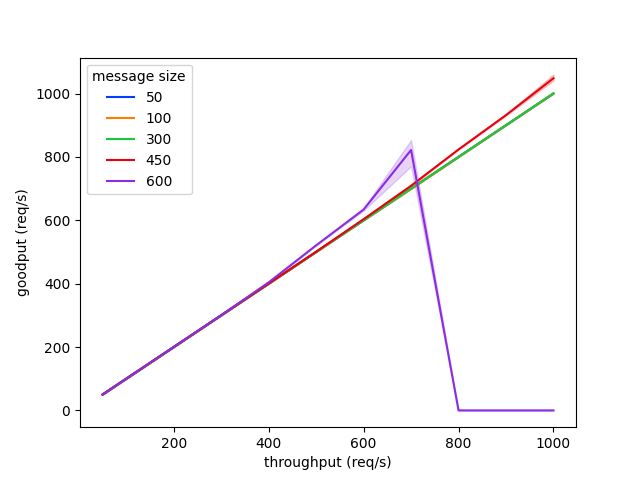
\includegraphics[scale=0.75]{dummy_throughputgoodput.png}
\end{figure}

\begin{figure}[h!]
\centering
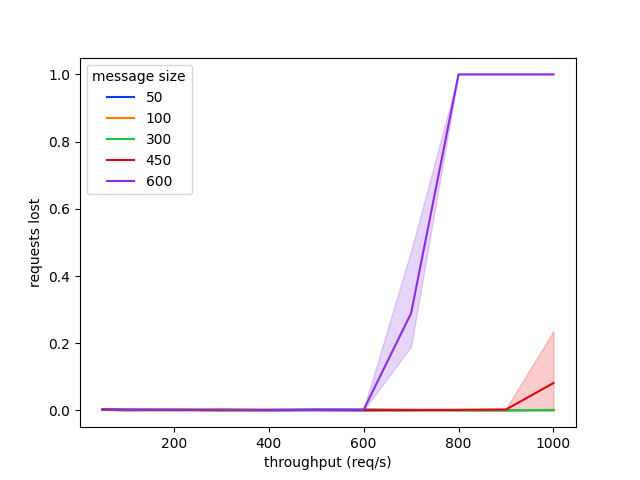
\includegraphics[scale=0.75]{dummy_throughputlost.png}
\end{figure}

The figures demonstrate that the framework has a severe drop in performance when sending large messages. For a message size of 600 the goodput goes to zero as the throughput increases, meaning that no messages are being responded to.

% https://seaborn.pydata.org/tutorial/color_palettes.html
[maybe add goodput / latency graph once it is in a reasonable state! ***]

\subsection{Tezos Cryptography} \label{tezosbenchmark}
I profiled the important functions of the library with Jane Street's Core\_bench module. Core\_bench is a micro-benchmarking library used to estimate the cost of operations in OCaml, it runs the operation many times and uses linear regression to try to reduce the effect of high variance between runs.

\begin{table}[!h]
	\centering
	\begin{tabular}{|l|r|}
	\hline
	Function                 & Time (µs) \\ \hline
	Sign                     & 427.87   \\
	Check                    & 1,171.77 \\
	Aggregate (4 sigs)       & 302.90   \\
	Aggregate check (4 sigs) & 1,179.25 \\
	Aggregate (8 sigs)       & 605.38   \\
	Aggregate check (8 sigs) & 1,180.61 \\ \hline
	\end{tabular}
\end{table}
% ┌─────────────┬────────────┬─────────┬──────────┬──────────┬────────────┐
% │ Name        │   Time/Run │ mWd/Run │ mjWd/Run │ Prom/Run │ Percentage │
% ├─────────────┼────────────┼─────────┼──────────┼──────────┼────────────┤
% │ sign        │   427.87us │ 144.00w │          │          │     36.24  │
% │ check       │ 1_171.77us │  75.00w │          │          │     99.25  │
% │ agg_4       │   302.90us │ 484.00w │    0.15w │    0.15w │     25.66  │
% │ agg_check_4 │ 1_179.25us │  75.00w │          │          │     99.88  │
% │ agg_8       │   605.38us │ 944.00w │    0.35w │    0.35w │     51.28  │
% │ agg_check_8 │ 1_180.61us │  75.00w │          │          │    100.00  │
% └─────────────┴────────────┴─────────┴──────────┴──────────┴────────────┘